\documentclass{article}
\usepackage[utf8]{inputenc}

\title{¿Como mejorar la calidad de las mallas?}
\author{Brayan Valdez Quispe}
\date{December 2018}

\usepackage{natbib}
\usepackage{graphicx}

\begin{document}

\maketitle

\section{Resumen}
La optimización de mallas puede ser muy útil en cualquier campo ya que lo que más se quiere en cualquier parte del mundo ya sea negocio u otro ámbito es reducir los costos y optimizar las ganancias, como ejemplo tenemos los productos que se guardan en un depósito, estos pueden ser colocados en cualquier parte del depósito pero en caso si queremos optimizar cada medida con el que cuenta los depósitos aplicamos la optimización de mallas y estos reducirán los espacios para que cada centímetro de producto encaje correctamente uno junto al otro y así optimizar la capacidad de productos que se pueden guardar en dicho depósito. \cite{alejandro2000metodos,juan2013optimizacion}

\section{Objetivo}
Este trabajo es una propuesta de aplicar método de optimización basado en mallas, cuyo fin es poder tener una mejor calidad de una métrica dada, es decir, la optimacion de medidas de un objeto y con esto podemos referenciarlo a un caso común que seria el mejoramiento de espacios. \cite{alejandro2000metodos}

\begin{figure}[h!]
\centering
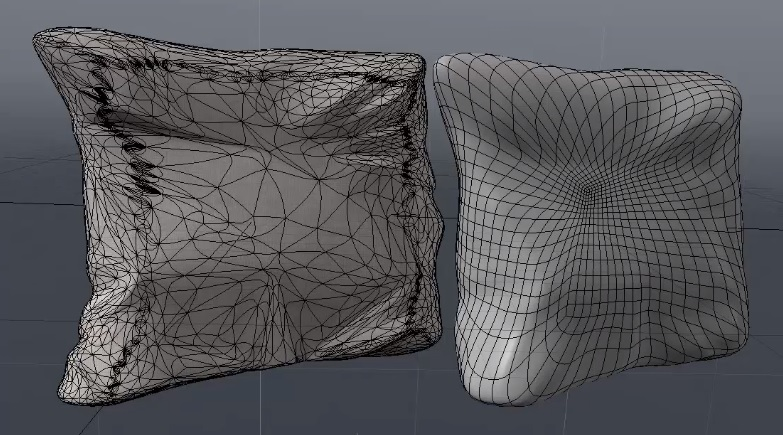
\includegraphics[width=9cm]{MallaOptimizada}
\caption{Malla Optimizada}
\label{fig:Malla Optimizada}
\end{figure}

\section{Metodología}
Encontramos tres metodologias para poder desarrollar la optimizacion de mallas, estas son mallas estructurada, mallas no estructurada y malla multibloque. \cite{alejandro2000metodos,martinez1991optimizacion}

\subsection{Metodología Estructurado}
Estas se utilizan fundamentalmente en elementos 2D y 3D, apartir de estos se van generando triangulos y tetraedos respectivamente. En esta podemos encontramos los métodos algebraicos, métodos basados en EDPs, métodos de superposición-deformación de retícula, métodos de crecimiento estructurado. \cite{alejandro2000metodos,Byron2014optimzacion}

\begin{figure}[h!]
\centering
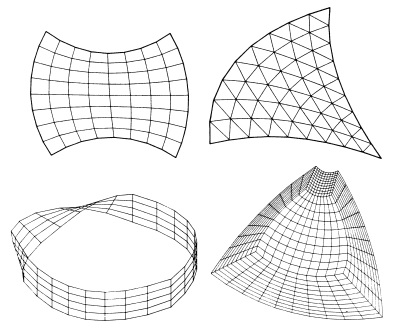
\includegraphics[width=10cm]{MallaAlgebraica}
\caption{Malla generada mediante Métodos Algebraicos}
\label{fig:Malla Algebraica}
\end{figure}

\subsection{Metodología No Estructurado}
Son aplicaciones más generales que las estructuradas, los más empleados en las prácticas se pueden dividir entre aquéllos que parten de una distribución determinada de nodos y únicamente se ocupan de obtener una conectividad adecuada, y aquellos otros en los que nodos, aristas y elementos o nodos, aristas, caras y elementos se generan conforme la malla va creciendo. Al buscar una conexión óptima de modo que los elementos presenten una buena relación de aspectos, esta triangulación óptima está garantizada si se emplea el método de Delaunay-Voronoï. \cite{alejandro2000metodos}

\begin{figure}[h!]
\centering
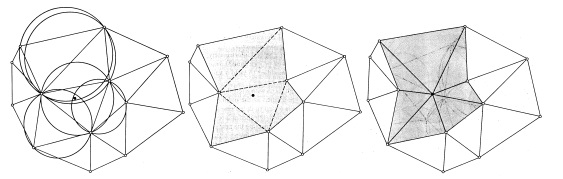
\includegraphics[width=12cm]{MallaDelaunay-Voronoi}
\caption{Triangulación de Delaunay}
\label{fig:Malla Delaunay}
\end{figure}

\subsection{Metodología Multibloque}
La metodología multibloque representa una solución para la creación de mallas de geometrías complejas para las que los métodos descritos previamente no generan resultados satisfactorios o fallan. La idea
básica consiste en la división del dominio en bloques de topología más sencilla. \cite{bugeda1990utilizacion,perazzo2006avances}

\begin{figure}[h!]
\centering
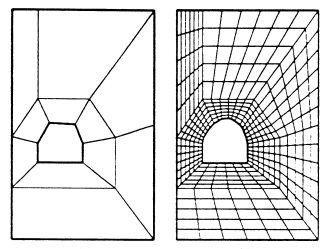
\includegraphics[width=10cm]{MallaMultibloque}
\caption{Generacion de Malla Multibloque}
\label{fig:Malla Multibloque}
\end{figure}

\bibliographystyle{plain}
\bibliography{references}
\end{document}
